\documentclass[a4paper,11pt]{article}

\usepackage[margin=3cm]{geometry}
\usepackage{amsfonts}
\usepackage{amsmath}
\usepackage{amssymb}
\usepackage{graphicx}

\usepackage[utf8]{inputenc}
%\usepackage[cp1250]{inputenc}
\usepackage[polish]{babel}
\usepackage[T1]{fontenc}


%----------------------
\def\\{\hfill\break}


%----------------------
\title{Projekt Egzaminacyjny}
\author{Maria Koren, Julian Jaroszyński}
\date{Listopad-Grudzień 2023}

\begin{document}
\maketitle
\newpage
\tableofcontents{}
\newpage

\section{Wstęp}
W tym projekcie reprezentowana jest analiza danych spółek KMR.UK (Kenmare Resources Plc) oraz JJB (Jujubee S.A)

Kenmare Resources plc to uznana firma wydobywcza, która zarządza kopalnią minerałów tytanu Moma położoną na północno-wschodnim wybrzeżu Mozambiku.
Kopalnia prowadzi produkcję komercyjną od 2009 roku i jest uznawana za głównego dostawcę produktów z piasku mineralnego dla klientów na całym świecie, działających w ponad
15 krajach.

Jujubee S.A. to studio deweloperskie zajmujące
się tworzeniem gier wideo, które ma swoim koncie
takie tytuły jak: „FLASHOUT 3D”, „Suspect in
Sight”, „Take Off – The Flight Simulator”,
strategię czasu rzeczywistego „Realpolitiks”, grę
przygodowo-dokumentalną „KURSK” oraz „Deep Diving
Simulator”. Studio zostało założone przez byłych
pracowników CD Projekt RED, Traveller’s Tales oraz
Inifinite Dreams. Celem firmy jest tworzenie niesamowicie
grywalnych i doskonale wyglądających gier na wszystkie
istotne platformy sprzętowe, takie jak iOS (iPhone,
iPod, iPad), Android, Mac, PC i konsole. Jujubee jest
spółką notowaną na rynku NewConnect (JJB).


\section{Analiza cen spółek}
\subsection{Analiza cen spółki KMR.UK}
\subsubsection{Wykres kursów zamknięcia pokazujący zmiany w czasie oraz
histogram}

Zrobiono wykres  kursu zamknięcia pokazujący zmiany w czasie, rysunek \ref{fig:cena_podcaz_zamkn}

\begin{figure}[h]
  \centering
  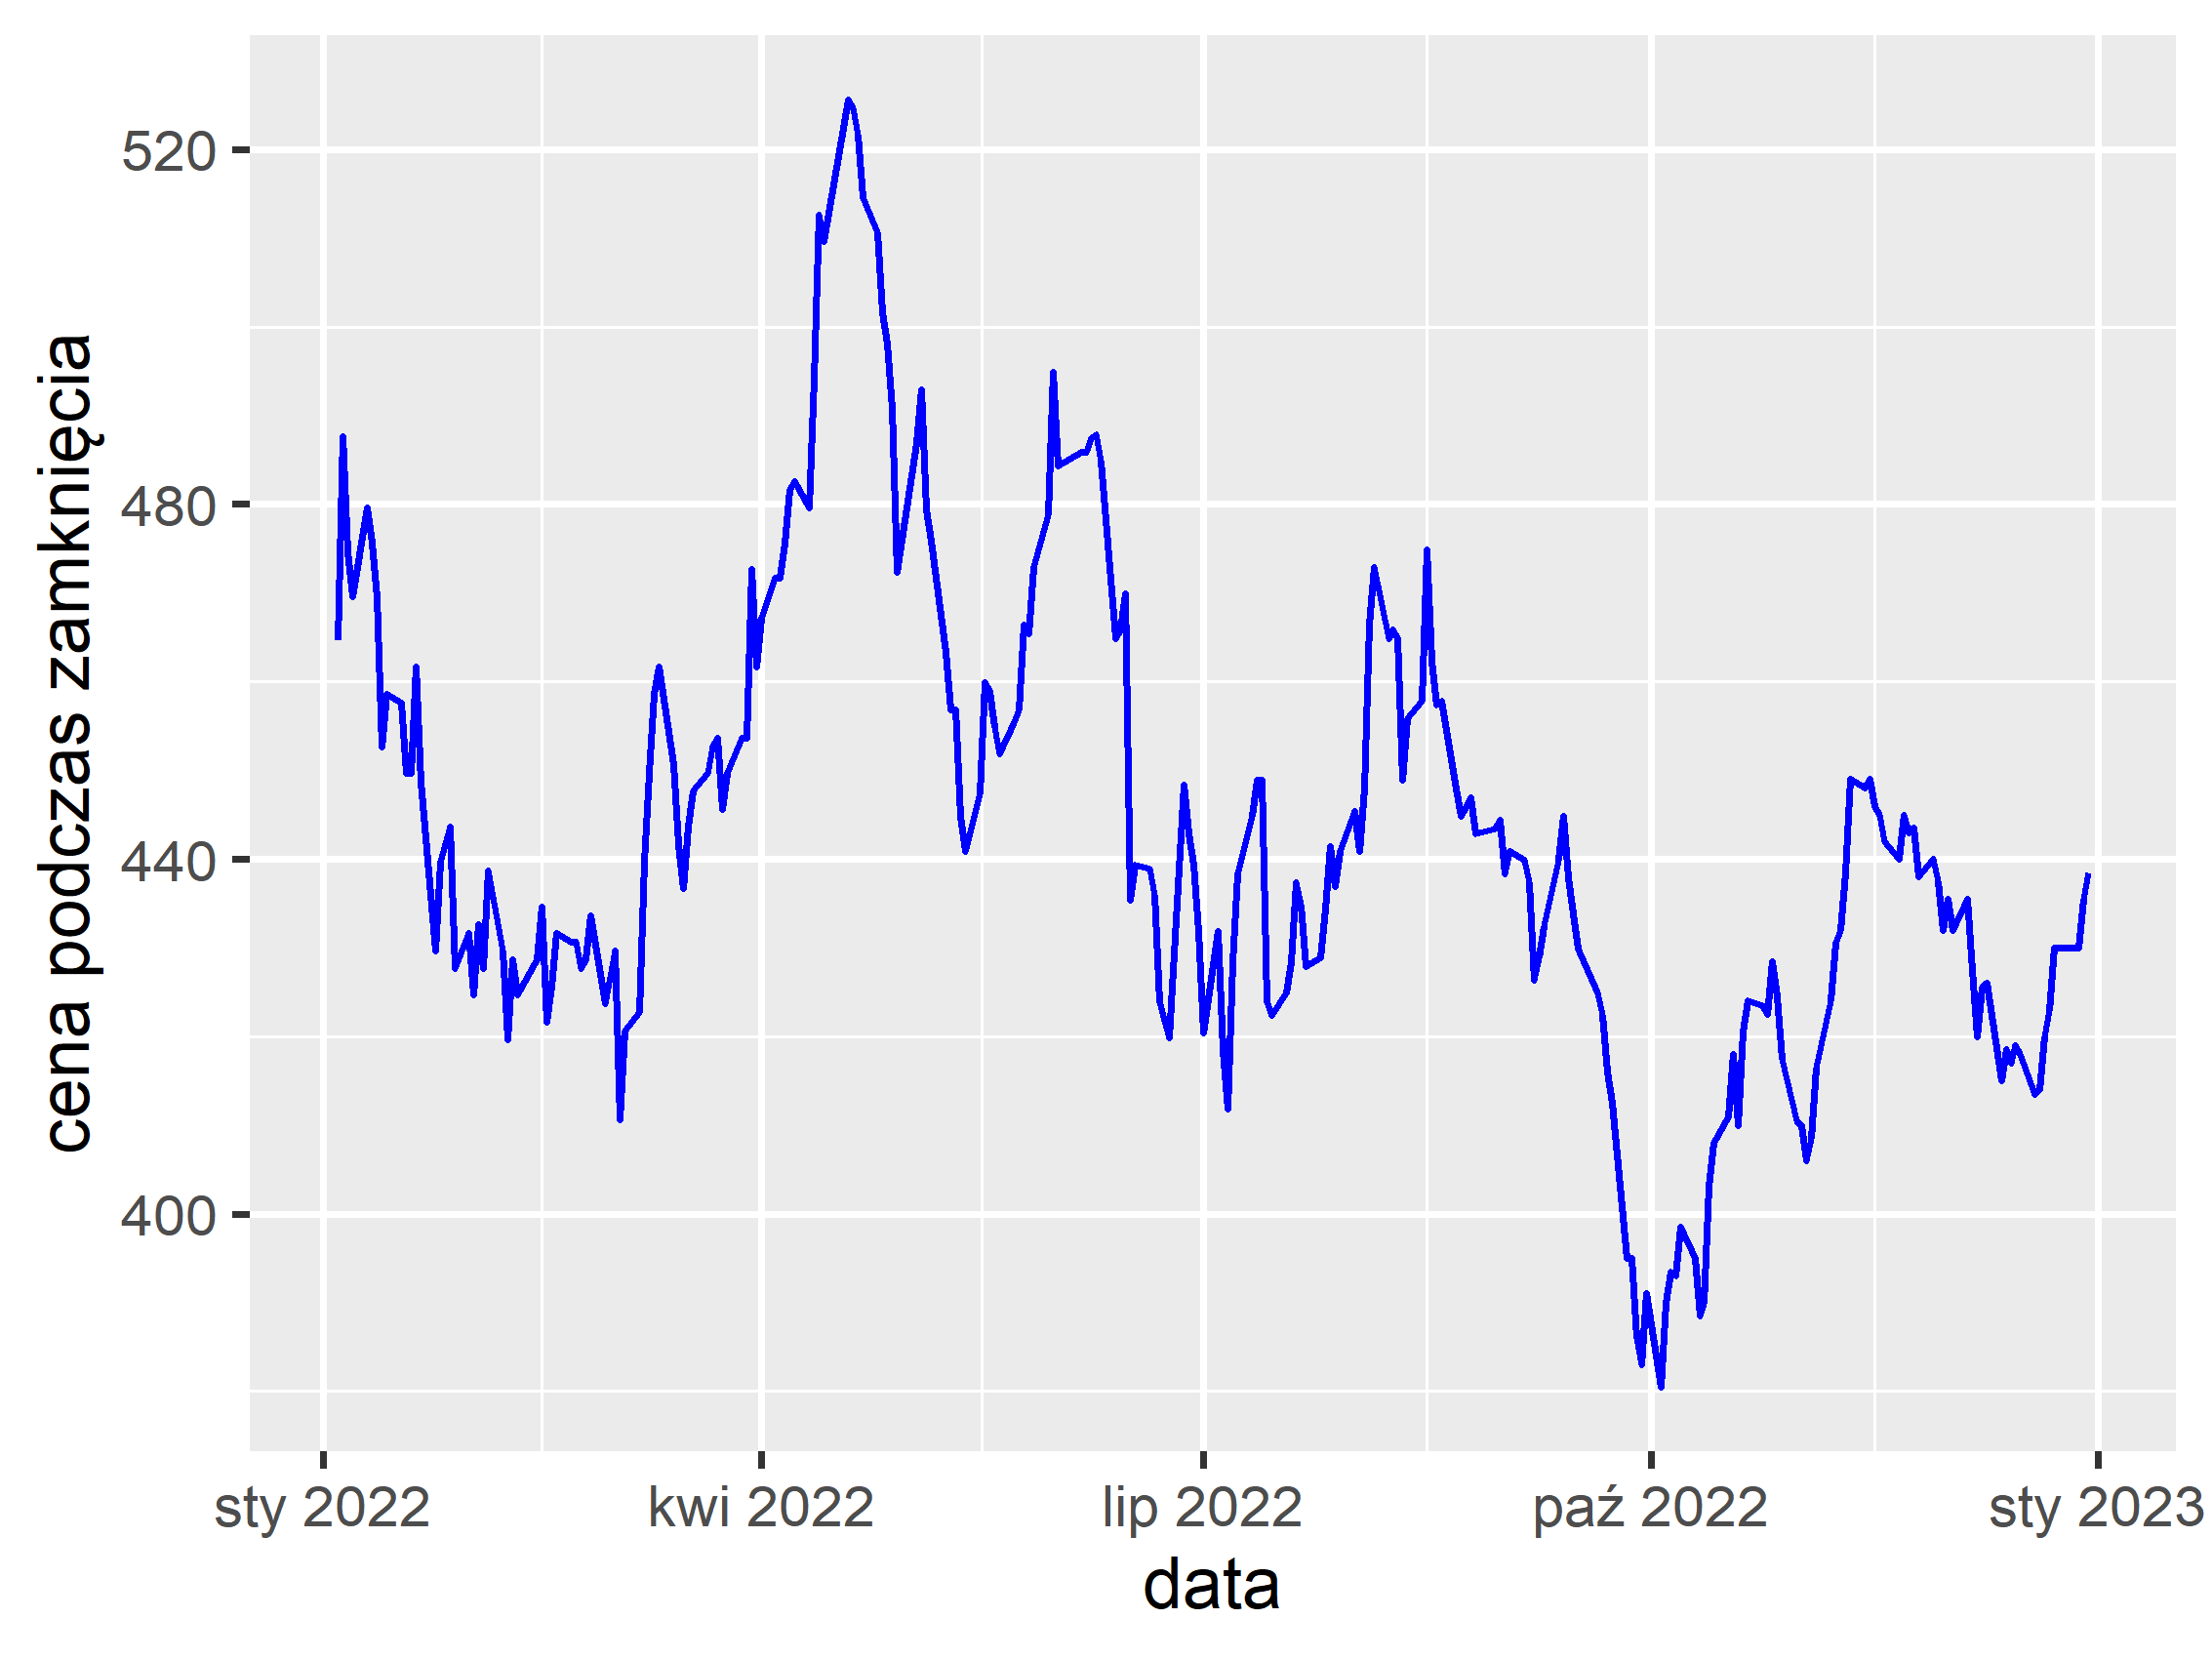
\includegraphics[width=10cm]{cena_poczas_zamkn.png}
  \caption{Cena podczas zamknięcia}
  \label{fig:cena_podcaz_zamkn}
\end{figure}

Oraz histogram, pokazujacy liczebność danych, rysunek \ref{fig:histogram}
\newpage
\begin{figure}[h]
  \centering
  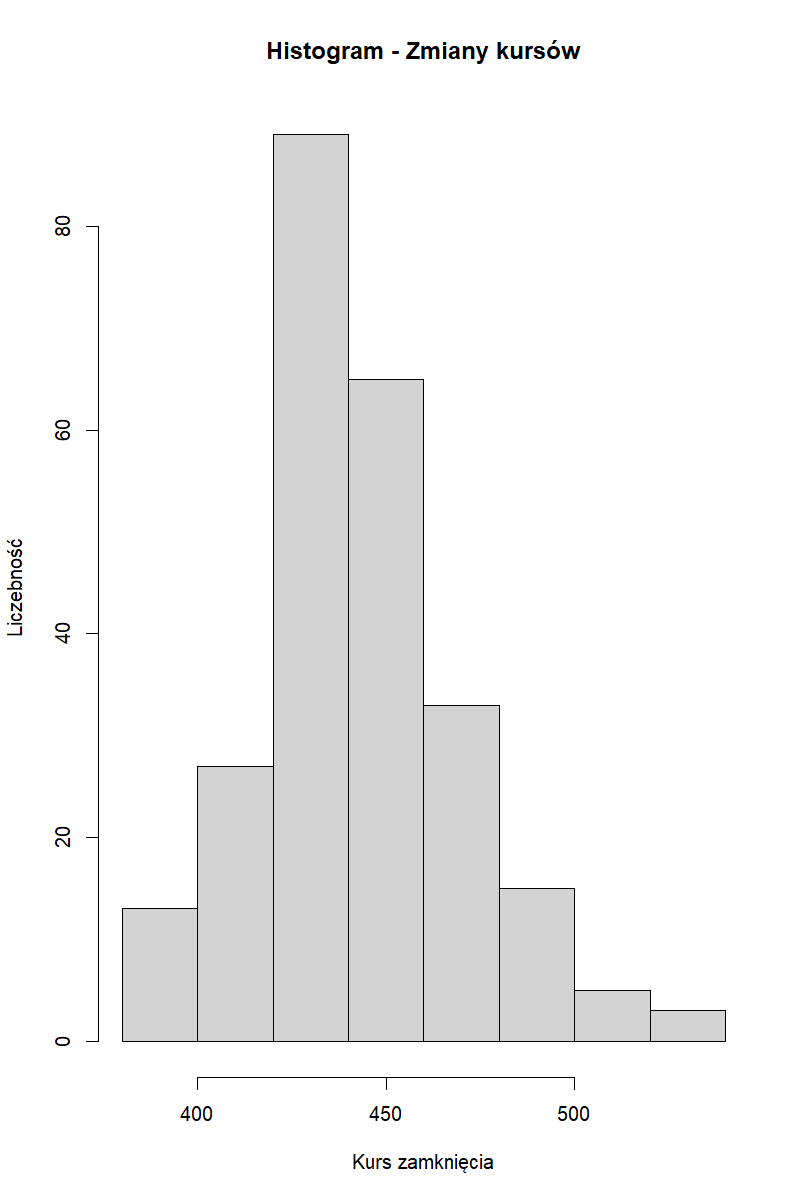
\includegraphics[width=10cm]{histogram.png}
  \caption{Histogram danych}
  \label{fig:histogram}
\end{figure}


\subsubsection{Statystyki opisowe}

Zostały obliczone nastepujące statystyki opisowe: średnia, odchylenie standardowe, skośność oraz kurtoza

Wyniki statystyk znajdują się w poniższej tabeli \ref{tab:statystyki_opisowe}

\begin{table}[h]
  \centering
  \begin{tabular}{|c|c|c|c|c|}
    \hline
     & $\bar{x}$ & odch. st. & skośność & kurtoza  \\
    \hline
    akcje & 442.8741 & 26.7262 & 3.574323 & 0.52783 \\
    \hline

    \hline
  \end{tabular}
  \caption{Statystyki opisowe}
  \label{tab:statystyki_opisowe}
\end{table}

\paragraph{Interpretacja wyników}
\begin{itemize}
  \item Otrzymana skośność mówi o przewadzę wartości wyższych (wartość skośności powyżej zera)
  \item  Otrzymana kurtoza mówi cieńszych ogonach niż rozkład normalny (bardziej płaski) (wartość kurtozy mniej niż 3)

\end{itemize}


\subsubsection{Estymacja parametrów trzech rozkładów korzystając z estymatora największej wiarygodności (MLE)}

Wyestymowano wyniki trzech rozkładów: normalnego, log-normalnego oraz rozkładu Weibulla za pomocą estymatora MLE. Wyżej wymienione wykresy dodano do wcześniejszego histogramu, co widać za rysynku \ref{fig:histogram_wykresy}


\begin{figure}[h]
  \centering
  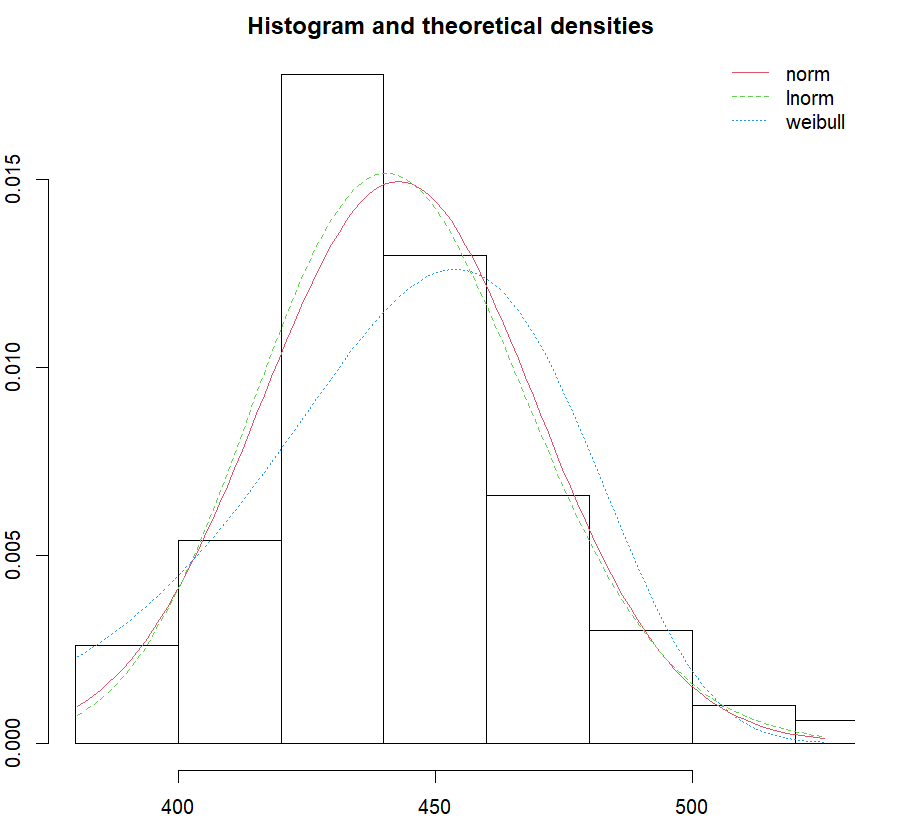
\includegraphics[width=10cm]{histogram_z_wykresami.png}
  \caption{Histogram wraz z estymowanami rozkładami}
  \label{fig:histogram_wykresy}
\end{figure}

Wyniki estymacji parametrów są przedstawione w tabeli \ref{wyniki_estymacji}
\begin{table}[h]
  \centering
  \begin{tabular}{|c|c|c|}
    \hline
     & $\mu$ & $\sigma$   \\
    \hline
    normalny & 442.8741 & 26.67269  \\
    \hline

    \hline
     & $\mu$ & $\sigma$   \\
    \hline
    log-normalny & 6.091499 & 0.05957788  \\
    \hline

    \hline
     & $a$ & $\sigma$   \\
    \hline
    weibulla & 15.61307 & 455.8914  \\
    \hline
  \end{tabular}
  \caption{Wyniki estymacji parametrów}
  \label{wyniki_estymacji}

\end{table}



Te wyniki oznaczają, że zostały dopasowane następujące rozkłady:

\begin{itemize}
  \item $X \sim\ N(442.87, 26.67)$
  \item $X \sim\ LN(6.09, 0.059)$
  \item $X \sim\ W(15.61, 455.89)$

\end{itemize}

\subsubsection{Wykresy diagnostyczne}
Zostały zrobione wykresy diagnostyczne qq-plot (rysunek \ref{fig:qqplot}) oraz cdf (rysunek \ref{fig:cdf})

\begin{figure}[htb]
  \centering
  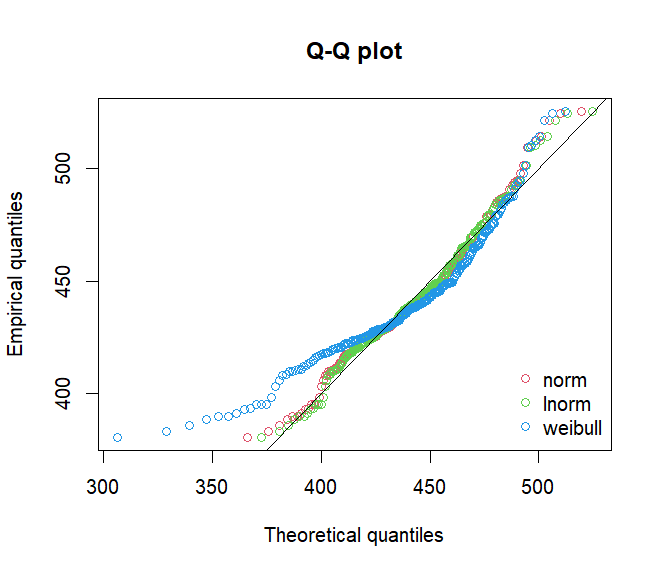
\includegraphics[width=9cm]{qqplot.png}
  \caption{Wykres qq-plot}
  \label{fig:qqplot}
\end{figure}

\begin{figure}[htb]
  \centering
  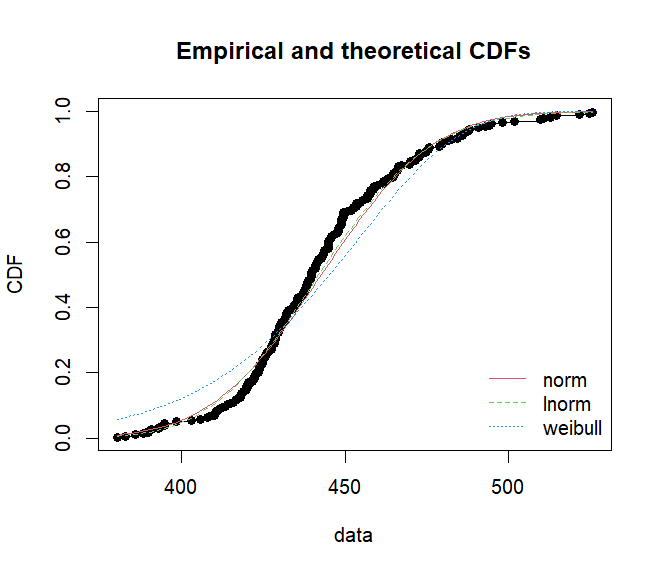
\includegraphics[width=9cm]{cdf.png}
  \caption{Wykres cdf}
  \label{fig:cdf}
\end{figure}

\begin{itemize}
  \item Wykres qq-plot
  
 Jest to wykres kwantyl-kwantyl, na osi pionowej są kwantyle teoretyczne, na osi   poziomowej są kwantyle empiryczne. Kwantyl rzędu $\alpha$  $\in$ (0, 1) zmiennej losowej ciągłej $X$ to taka liczba q, dla której prawdopodobieństwo, że zmienna $X$ przyjmuje   wartości mniejsze lub równe q jest równe $\alpha$.
      
  Najlepiej jest gdy te kwantyle są takie same bądź bardzo blizkie siebie. Dlatego   najlepszym rozkładem  jest najbliższy do prostej $y=x$. W rozważanym przykład takim   jest wykres log-normalny $X \sim\ LN(6.09, 0.059)$
  \item Wykres CDF

  Funkcja rozkładu kumulacyjnego (CDF, Cumulative Distribution Function) to graficzna reprezentacja kumulatywnej dystrybuanty danej zmiennej losowej. CDF dla danej wartości $x$ to prawdopodobieństwo, że zmienna losowa przyjmuje wartość mniejszą lub równą $x$. Czarnym zaznaczone są dane empiryczne. Najlepszym wykresem jest mający teorytyczne dane najbliższe do danych empirycznych. W rozważanym przykładzie takim wykresem jest log-normalny $X \sim\ LN(6.091, 0.059)$
\end{itemize}

Na podstawie wykresów diagnostycznych najlepszym rozkładem jest rozkład logarytmiczno-normalny

\paragraph{Analiza wartości statystyk KS, CM i AD oraz kryteria informacyjne AIC i BIC}
\\
Bazując wyłącznie na wykresach diagnostycznych, nie jest możliwe wybranie jednego najlepszego wykresu. Dlatego skorzystano ze statystyk Kołmogorowa-Smirnowa, Cramera-von-Misesa, Andersona-Darlinga, a także z kryteriów informacyjnych AIC (Akaike's Information Criterion) oraz BIC (Bayesian Information Criterion)

Wartości ze statystyk KS, CM, AD są umieszczone w tabeli \ref{tab:statystyki}. Wartości kryteriów AIC, BIC w tabeli \ref{tab:kryteriaInf}


\begin{table}[htb]
  \centering
  \begin{tabular}{|c|c|c|c|}
    \hline
     & normalny & log-normalny & weibull  \\
    \hline
    Kolmogorov-Smirnov & 0.09168955 & 0.0798396 & 0.138442\\
    \hline
    Cramer-von Mises & 0.3613063 & 0.2485924 & 1.257677 \\
    \hline
    Anderson-Darling & 2.005469 & 1.412547 & 7.416593 \\
    \hline
  \end{tabular}
  \caption{Statystyki}
  \label{tab:statystyki}
\end{table}


\begin{table}[htb]
  \centering
  \begin{tabular}{|c|c|c|c|}
    \hline
     & normalny & log-normalny & weibull  \\
    \hline
    Akaike's Information Criterion & 2355.289 & 2348.983 & 2415.692\\
    \hline
    Bayesian Information Criterion & 2362.332 & 2356.026 & 2422.735 \\
    \hline
  \end{tabular}
  \caption{Kryteria informacyjne}
  \label{tab:kryteriaInf}
\end{table}

Ponieważ statystyki są oparte na porównaniu odległości dystrybuant, najlepszym rozkładem jest ten, który jest najbliżej do danych teorytycznych (ma najmniejszą odległość), czyli ma najmniejszą wartość statystyki. W kryteriach informacyjnych za najlepszy rozkład również jest uważany rozkład, mający najmniejszą wartosć kryteria. W rozważanym przykładzie takim rozkładem jest rozkład log-normalny $X \sim\ LN(6.09, 0.059)$

\subsubsection{Testowanie hipotezy o równości rozkładów, wykorzystując  statystykę KS}

Zrobiona hipoteza H0: $F=LN(6.09, 0.0595)$ przeciwko hipotezie H1: F nie jest rowny $LN(6.09, 0.059)$

Zgenerowano $N=10000$ probek licznosci $n$ (równej ilości danych) z rozkładu $F0=LN(6.09, 0.059)$ wybranego wcześniej jako najlepszego rozkładu i obliczono odleglość dystrybuant empirycznych od rozkladu F0 (wartosc statystyki Dn)

Obliczona również wartość statystyki dla rzeczywustych danych

Rysowany jest histogram statystyk testu KS uzyskanych z danych losowych, a także dodany jest punkt dla statystyki testu KS uzyskanej z rzeczywistych danych dla porównania danych rzeczywistych z danymi losowymi tego rozkładu


\begin{figure}[htb]
  \centering
  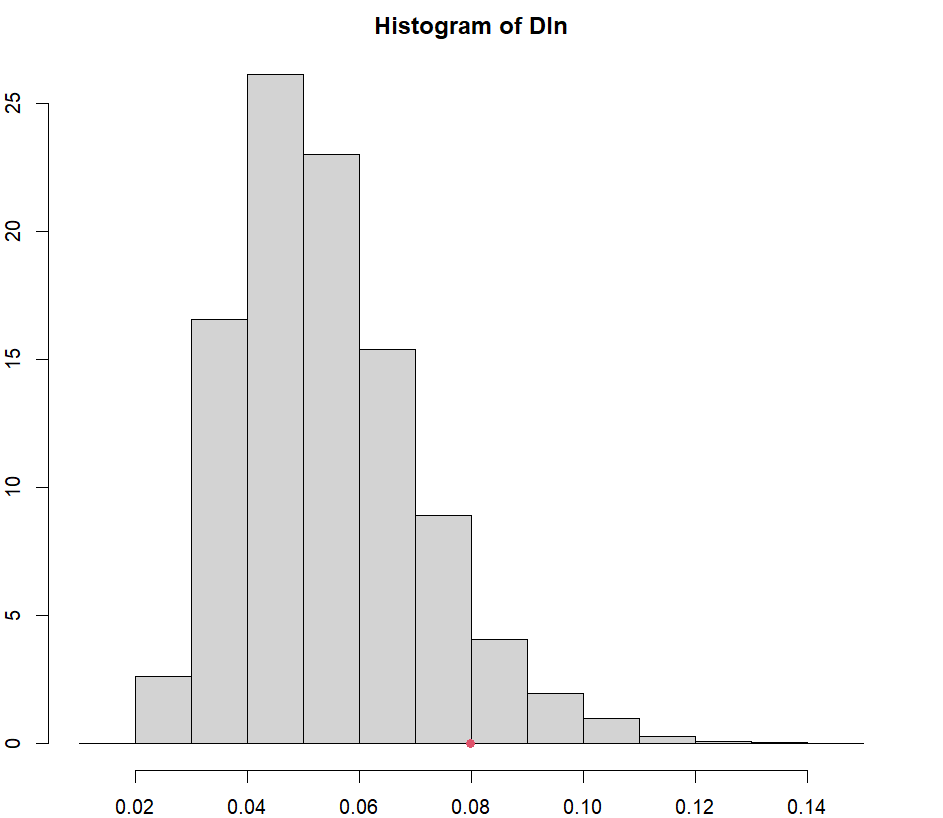
\includegraphics[width=9cm]{histogram_dane_teoryteczne.png}
  \caption{Histogram danych teorytycznych}
  \label{fig:hisT_dane_teor}
\end{figure}

Z wykresu widać, że wynik z danych rzeczywistych jest umieszczony w miejscu, gdzie dane losowe jeszcze są
\\

Ta statystyka zwraca 2 dane: odległość (wartość \textit{statistic}) oraz prawdopodobieństwo że wartości statystyki KS są takie same lub większe, gdy hipoteza zerowa jest prawdziwa

Wyniki tego testowania zostaną umieszczone w tabeli \ref{tab:wyniki_testowania}:

\begin{table}[htb]
  \centering
  \begin{tabular}{|c|c|}
    \hline
     statistic & p-value   \\
    \hline
     0.0798396  & 0.0827\\
    \hline
  \end{tabular}
  \caption{Wartość statystyki KS w testowaniu hipotezy}
  \label{tab:wyniki_testowania}
\end{table}


P-wartość informuje o prawdopodobieństwie uzyskania takiej samej lub bardziej ekstremalnej statystyki testu, niż ta, którą otrzymaliśmy z danych rzeczywistych (zakładając że dane pochodzą z tego samego rozkładu)

Ponieważ p-wartosć  p = 0.0827 > 0.05 zatem nie ma powodów odrzucenia hipotezy. Uzyskane wyniki potwierdzają wybraną hipotezę  o logarytmiczno-normalnym $LN(6.09, 0.059)$ rozkładzie danych


\subsection{Analiza cen spółki JJB}
\subsubsection{Wykres kursów zamknięcia pokazujący zmiany w czasie oraz histogram}

Wykres przedstawiający kursy zamknięcia firmy Jujubee S.A. (jjb) wraz z histogramem
\begin{figure}[h]
  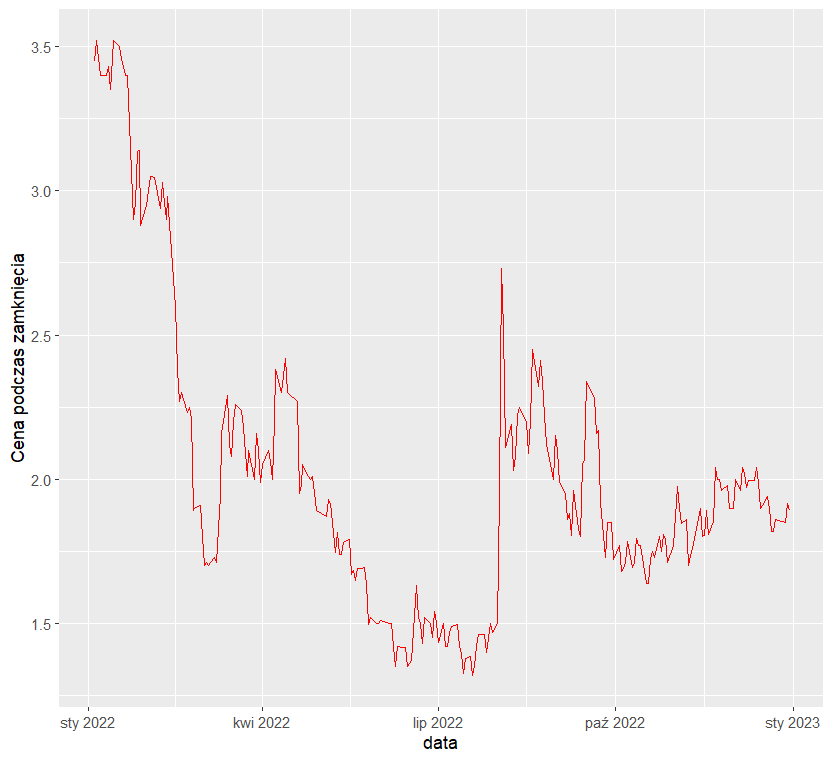
\includegraphics[width=5cm]{jjb_cena_podczas_zamkn.png}
  \caption{Cena podczas zamknięcia}
  \label{fig:jjb_cena_podcaz_zamkn}
\end{figure}

 
\begin{figure}[htb]
  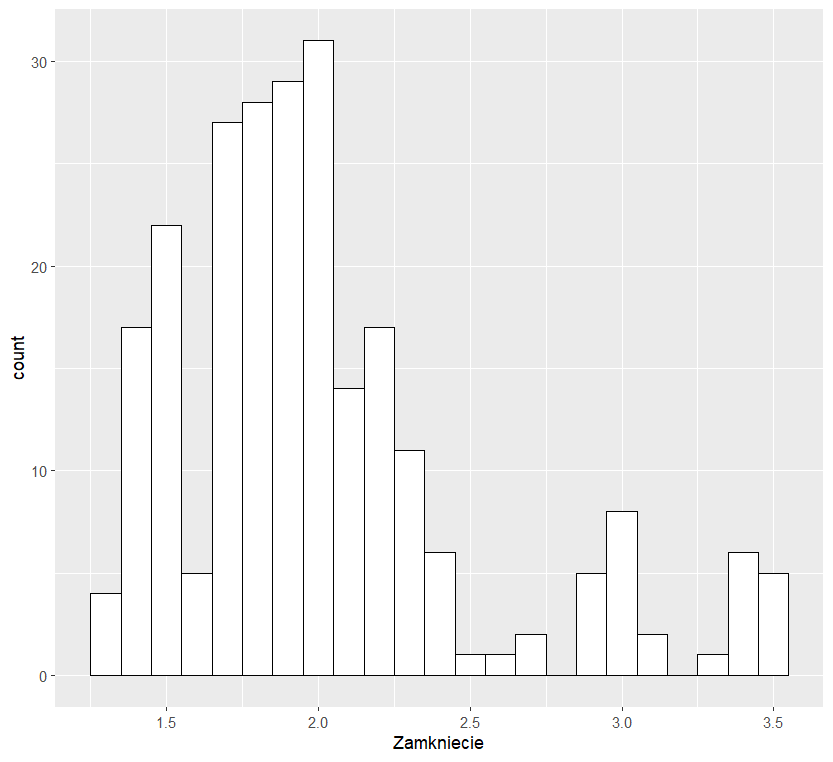
\includegraphics[width=5cm]{jjb_hist.png}
  \caption{Histogram danych}
  \label{fig:jjb_histogram}
\end{figure}
 
\subsubsection{Statystyki opisowe}

Jest to skośnść prawostronna (liczba jest dodatnia), oznacz to że jest
dużo przypadków mniejszych od średniej, firma miała parę dużych kursów
podbijających średnią;
Jest to rozkład leptokurtyczny, oznacz to że wartości są skoncentrowane
wokół śreniej oraz to że istnieje duża szansa na pojawienie się
odstających obserwacji
	\begin{table}[htb]
		\centering
		\renewcommand\tablename{Tabela}
		\begin{tabular}{|c|c|c|c|c|}
			\hline
			 & $\bar{x}$ & odch. st. & skośność & kurtoza \\
			\hline
			Akcja & 2.017201 & 0.5117912 & 1.319479 & 1.417186 \\
			\hline
		\end{tabular}
		\caption{statystyki opisowe}
		\label{tab:przyklad}
	\end{table}
\subsubsection{Estymacja parametrów trzech rozkładów korzystając z estymatora największej wiarygodności (MLE)}

Wyestymowano wyniki trzech rozkładów: normalnego, log-normalnego oraz rozkładu Weibulla za pomocą estymatora MLE. Wyżej wymienione wykresy dodano do wcześniejszego histogramu, co widać za rysynku \ref{fig:jjb_histogram_wykresy}

\begin{figure}[htb]
  \centering
  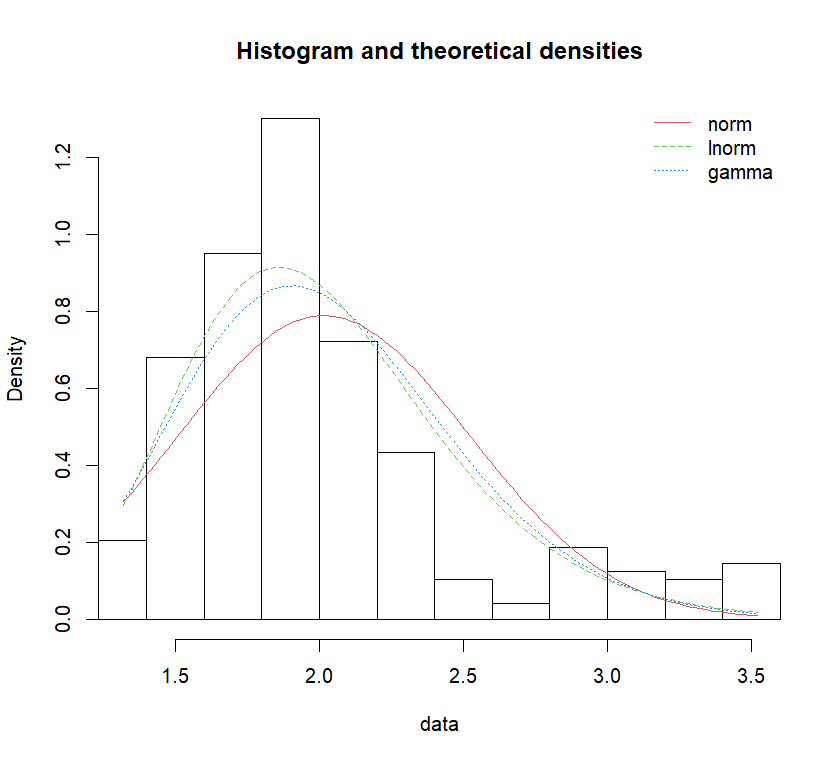
\includegraphics[width=10cm]{jjb_hist_wykresy.png}
  \caption{Histogram wraz z estymowanami rozkładami}
  \label{fig:jjb_histogram_wykresy}
\end{figure}

Parametry trzech rozkładów

	\begin{table}[htb]
		\centering
		\begin{tabular}{|c|c|}
			\hline
			& estymator \\
			\hline
			średnia & 2.0172008\\
			\hline
			sd & 0.5107625 \\
			\hline
		\end{tabular}
		\caption{parametry rozkładu normalnego}
	\end{table}
 \\
	\begin{table}[htb]
		\centering
		\begin{tabular}{|c|c|}
			\hline
			& estymator  \\
			\hline
			średnia & 0.6736043  \\
			\hline
			sdlog & 0.2306277 \\
			\hline
		\end{tabular}
		\caption{parametry rozkładów log-normalnego}
	\end{table}
 \\
	\begin{table}[htb]
		\centering
		\begin{tabular}{|c|c|}
			\hline
			& estymator  \\
			\hline
			kształt & 17.954308 \\
			\hline
			rate & 8.900479 \\
			\hline
		\end{tabular}
		\caption{parametry rozkładów gamma}
	\end{table}

 Te wyniki oznaczają, że zostały dopasowane następujące rozkłady:

\begin{itemize}
  \item $X \sim\ N(2.02, 0.51)$
  \item $X \sim\ LN(0.67, 0.23)$
  \item $X \sim\ \Gamma(17.95, 8.9)$

\end{itemize}

\subsubsection{Wykresy diagnostyczne}
Zrobiono wykresy diagnostyczne qqplot oraz cdf

\begin{figure}[htb]
  \centering
  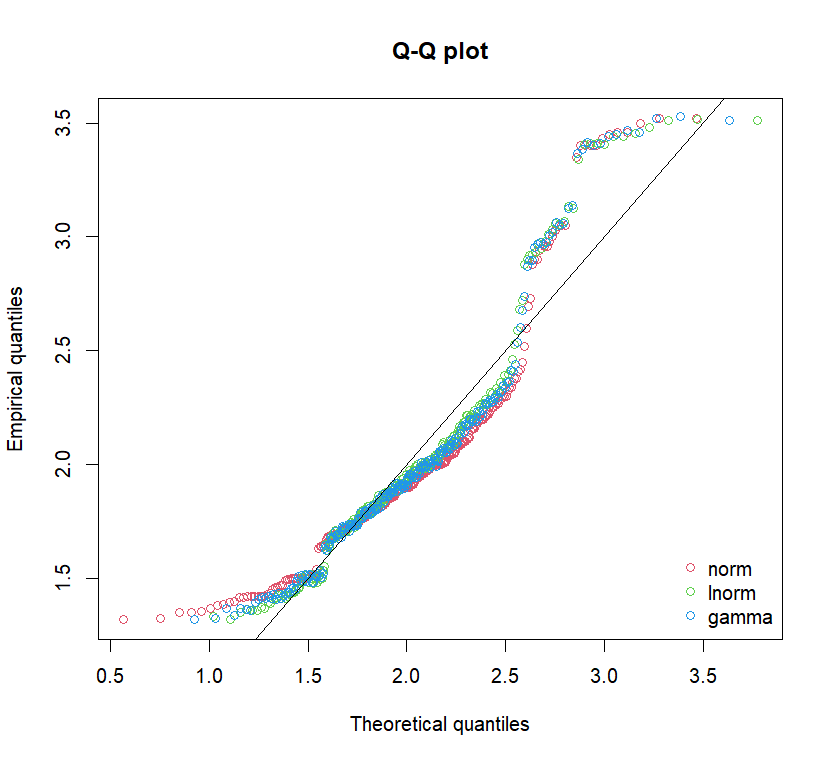
\includegraphics[width=9cm]{jjb_qqplot.png}
  \caption{Wykres qq-plot}
  \label{fig:jjb_qqplot}
\end{figure}

\begin{figure}[h]
  \centering
  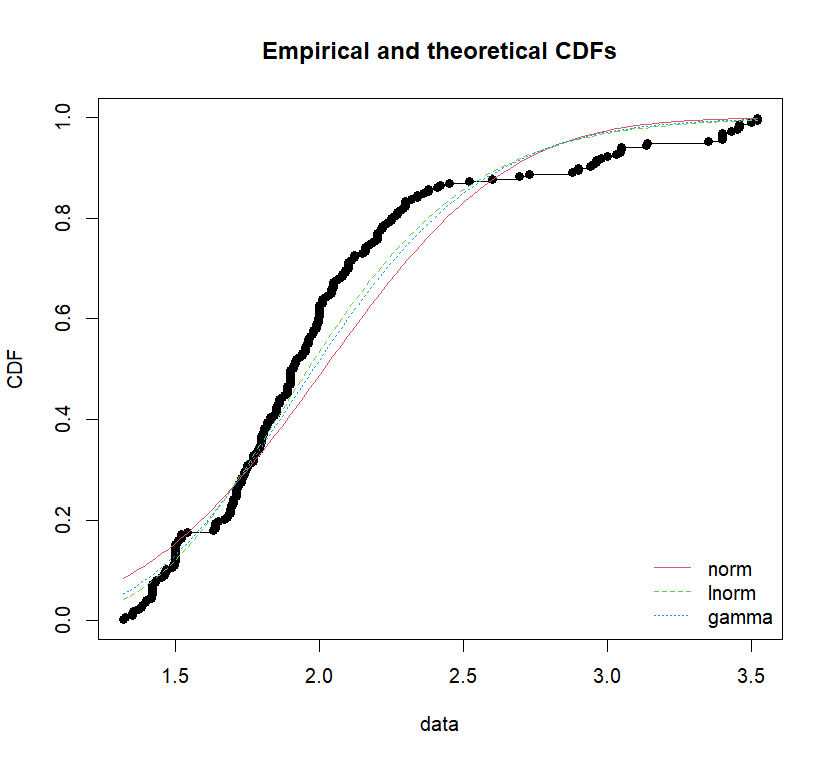
\includegraphics[width=9cm]{jjb_cdf.png}
  \caption{Wykres cdf}
  \label{fig:jjb_cdf}
\end{figure}

Na podstawie tych wykresów można wywnioskować że wykres
lnorm jest najlepiej opisujący kursy zamknięcia, ale aby to
dokładnie stwierdzić trzeba wykonać analizę statystyk KS,
CM i AD oraz kryteriów informacyjnych AIC i BIC

\paragraph{KS, CM, AD}
\\
Analiza dopasowania rozkładów za pomocą
testów Kolmogorova-Smirnova, Cramera-von Misesa i
Andersona-Darlinga pokazuje, że dla rozkładu normalnego
(norm), log-normalnego (lnorm) i rozkładu gamma (gamma)
wartości statystyk są odpowiednio 0.1465, 0.0946 i
0.1122 dla testu Kolmogorova-Smirnova, 1.5942, 0.5890
i 0.8612 dla testu Cramera-von Misesa, oraz 10.0248,
4.1675 i 5.7877 dla testu Andersona-Darlinga.
\begin{table}[htb]
\renewcommand\tablename{Tabela}
\centering
\begin{tabular}{|c|c|c|c|}
\hline
& norm & lnorm & gamma \\
\hline
Kolmogorov-Smirnov statistic & 0.1464534 & 0.09463034 & 0.1121969 \\
\hline
Cramer-von Mises statistic & 1.5941731 & 0.58899369 & 0.8611976 \\
\hline
Anderson-Darling statistic & 10.0247605 & 4.16749359 & 5.7876581 \\
\hline
\end{tabular}
\caption{Goodness-of-fit statistics}
\end{table}
\paragraph{AIC, BIC}
\\
Porównanie kryteriów doboru modelu, takich jak Akaike's
Information Criterion (AIC) i Bayesian Information
Criterion (BIC), wskazuje, że dla rozkładu normalnego
(norm), log-normalnego (lnorm) i rozkładu gamma (gamma)
wartości wynoszą odpowiednio 376.0498, 315.5450 i
331.6349 dla AIC, oraz 383.0847, 322.5800 i 338.6698
dla BIC.
\begin{table}[htb]
\renewcommand\tablename{Tabela}
\centering
\begin{tabular}{|c|c|c|c|}
\hline
& norm & lnorm & gamma \\
\hline
Akaike's Information Criterion & 376.0498 & 315.545 & 331.6349 \\
\hline
Bayesian Information Criterion & 383.0847 & 322.580 & 338.6698 \\
\hline
\end{tabular}
\caption{Goodness-of-fit criteria}
\end{table}

Na podstawie wyżej wymienonych statystyk najlepszym jest rozkład log-normalny $X \sim\ LN(0.67, 0.23)$


\subsubsection{Testowanie hipotezy o równości rozkładów, wykorzystując statystykę KS}

Zrobiona hipoteza H0: $F=LN(0.67, 0.23$ przeciwko hipotezie H1: F nie jest rowny $LN(0.67, 0.23)$. Do przetestowania hipotezy został użyty sposób Kolmogorova-Smirnova (KS), którego wynikiem jest: 0.3202. Ta wartość jest większa niż 0.05, przez co hipoteza zerowa jest potwierdzona
\begin{figure}[htb]
	\centering
	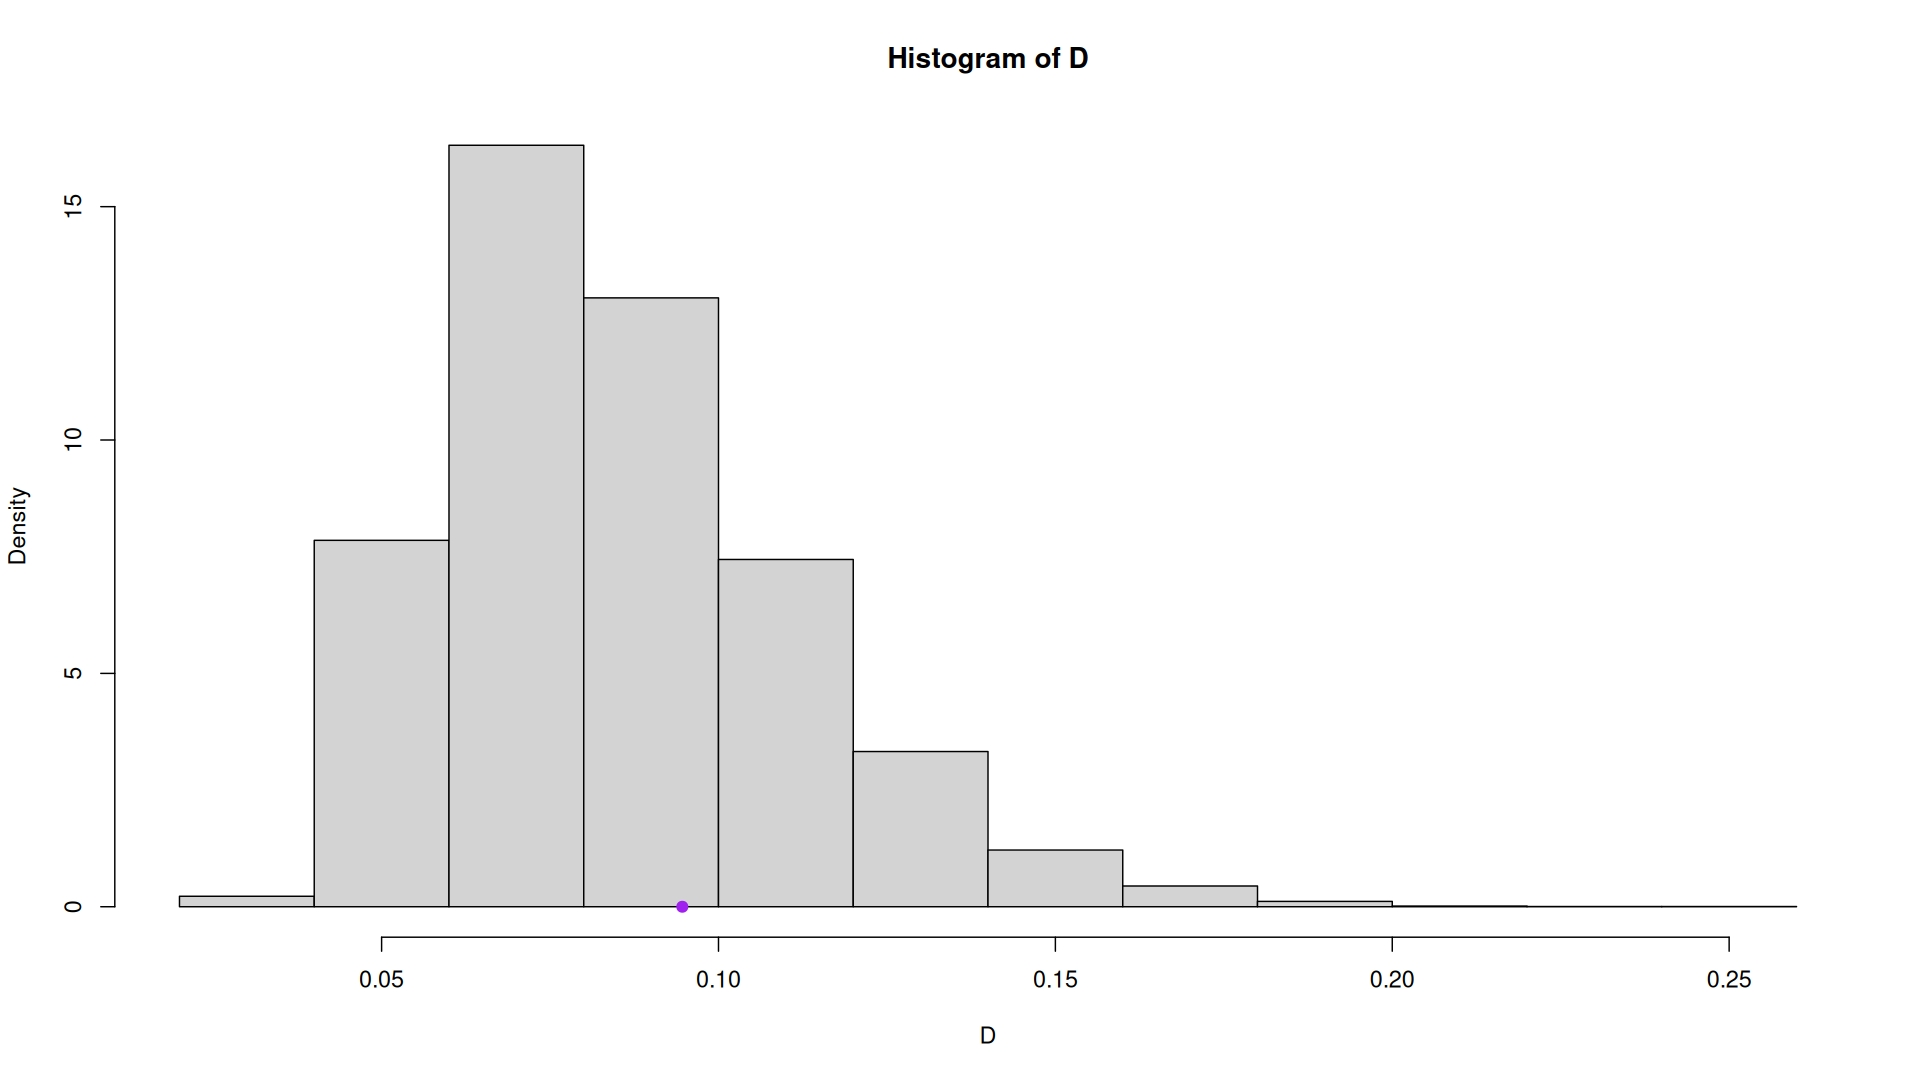
\includegraphics[width=5cm]{hist2.jpg}
	\caption{histogram metody ks}
\end{figure}

\pagebreak
\section{Analiza łącznego rozkładu log-zwrotów}
\subsection{Analiza rozkładów brzegowych}
\subsubsection{Analiza rozkładów brzegowych spółki KMR}

Na rysynkach \ref{fig:kmr_wykres_log} oraz \ref{fig:kmr_hist_log} są przedstawione odpowiednio wykresy log-zwrotów oraz histogram
\begin{figure}[htb]
	\centering
	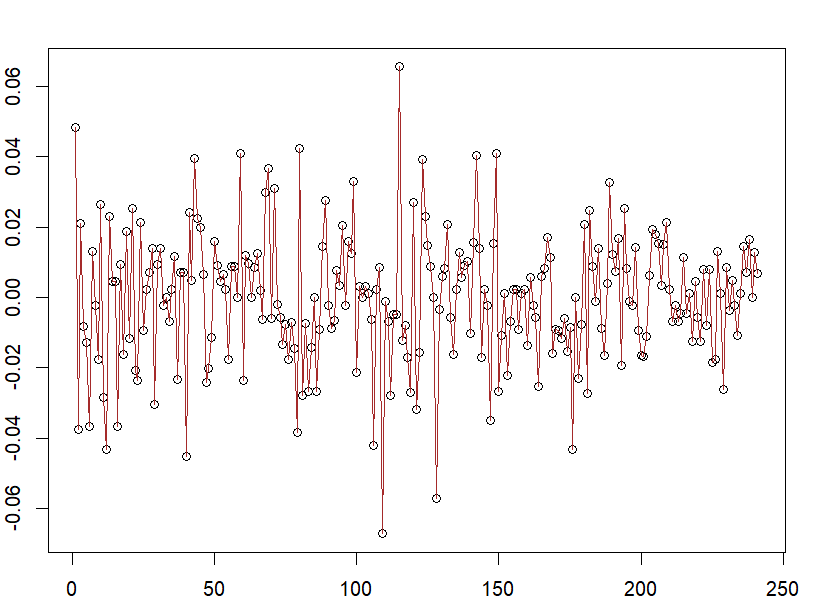
\includegraphics[width=10cm]{kmr_wykres_log.png}
        \label{fig:kmr_wykres_log}
	\caption{Wykres log-zwrotów spółki KMR}
\end{figure}

\begin{figure}[htb]
	\centering
	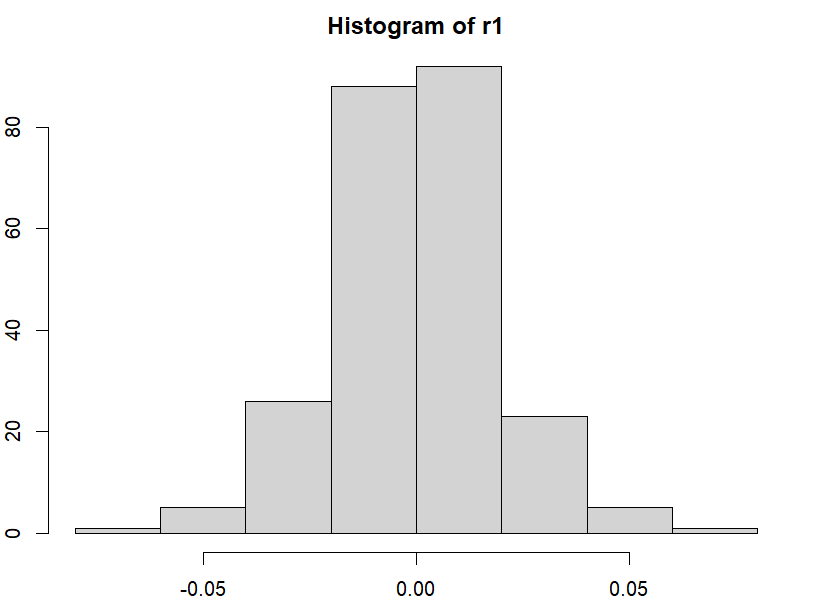
\includegraphics[width=10cm]{kmr_hist_log.png}
        \label{fig:kmr_hist_log}
	\caption{Wykres log-zwrotów spółki KMR}
\end{figure}

Został dopasowany do tych danych rozkład normalny $X \sim\ N(-0.0023, 0.018)$
\begin{figure}[htb]
	\centering
	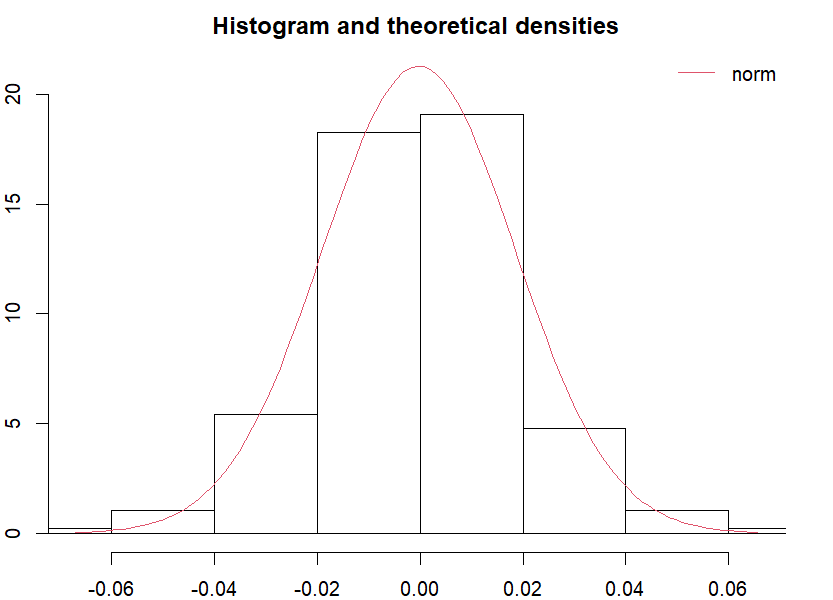
\includegraphics[width=10cm]{kmr_histW_log.png}
        \label{fig:kmr_histwykres_log}
	\caption{Wykres log-zwrotów wraz z dopasowanym rozkładem normalnym spółki KMR}
\end{figure}

Zrobiony wykres diagnostyczne cdf oraz qqplot, rysunki \ref{fig:kmr_qqplot_log}, \ref{fig:kmr_cdf_log.png}

\begin{figure}[htb]
	\centering
	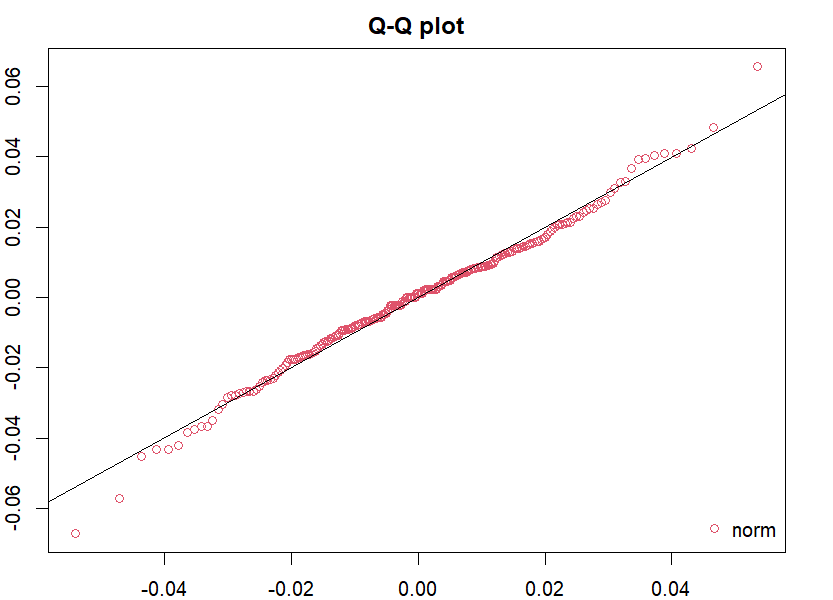
\includegraphics[width=10cm]{kmr_qqplot_log.png}
        \label{fig:kmr_qqplot_log}
	\caption{Wykres qqplot dla log-zwrotów spółki KMR}
\end{figure}

\begin{figure}[htb]
	\centering
	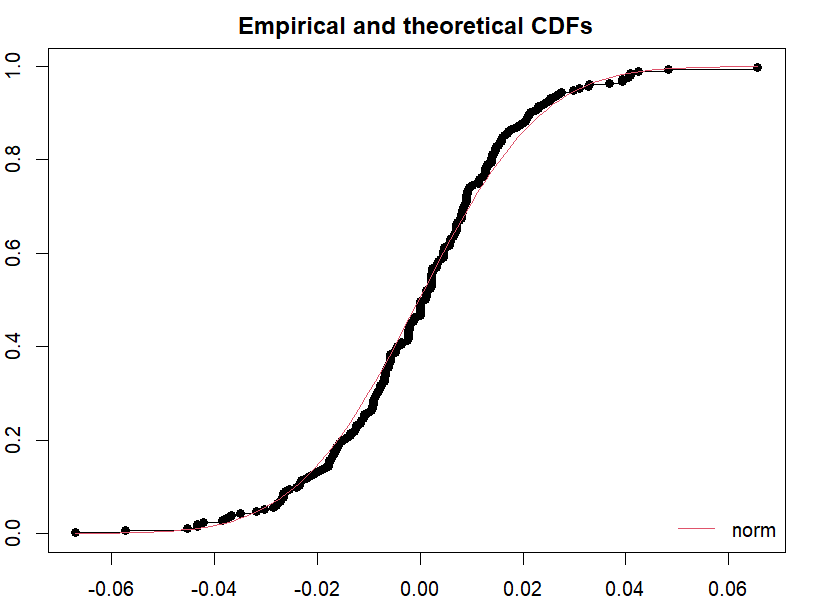
\includegraphics[width=10cm]{kmr_cdf_log.png}
        \label{fig:kmr_cdf_log.png}
	\caption{Wykres cdf dla log-zwrotów spółki KMR}
\end{figure}

Przeprowadzono również test równości metodą Monte-Carlo. Skorzystano ze statystyki Kolmogorova-Smirnova. Wynik p-value otrzymany w tym teście jest 0.5656, co oznacza przyjęcie hipotezy że rozklad log-zwrotów jest  $X \sim\ N(-0.0023, 0.018)$

\begin{figure}[htb]
	\centering
	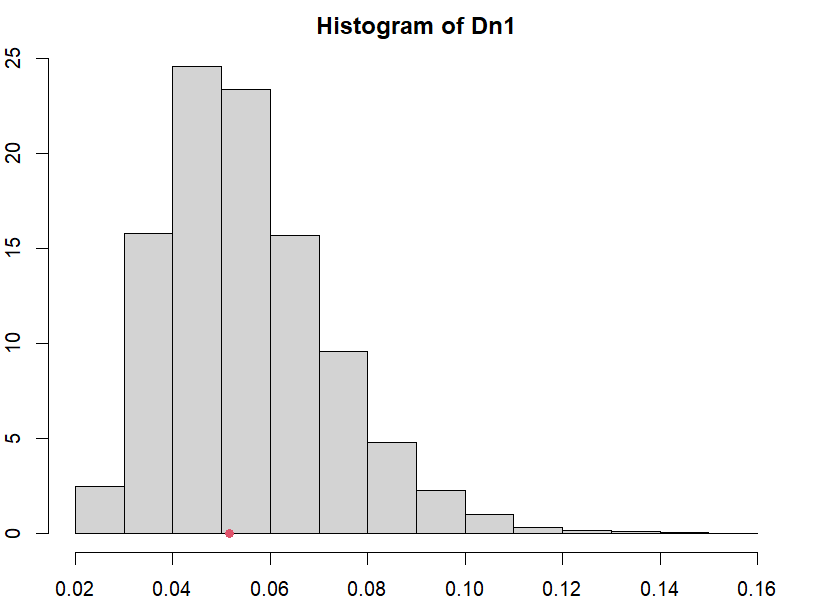
\includegraphics[width=10cm]{kmr_histMC.png}
        \label{fig:kmr_histMC}
	\caption{Histogram danych w teście }
\end{figure}

\subsubsection{Analiza rozkładów brzegowych spółki JJB}

Na rysynkach \ref{fig:jjb_wykres_log} oraz \ref{fig:jjb_hist_log} są przedstawione odpowiednio wykresy log-zwrotów oraz histogram
\begin{figure}[htb]
	\centering
	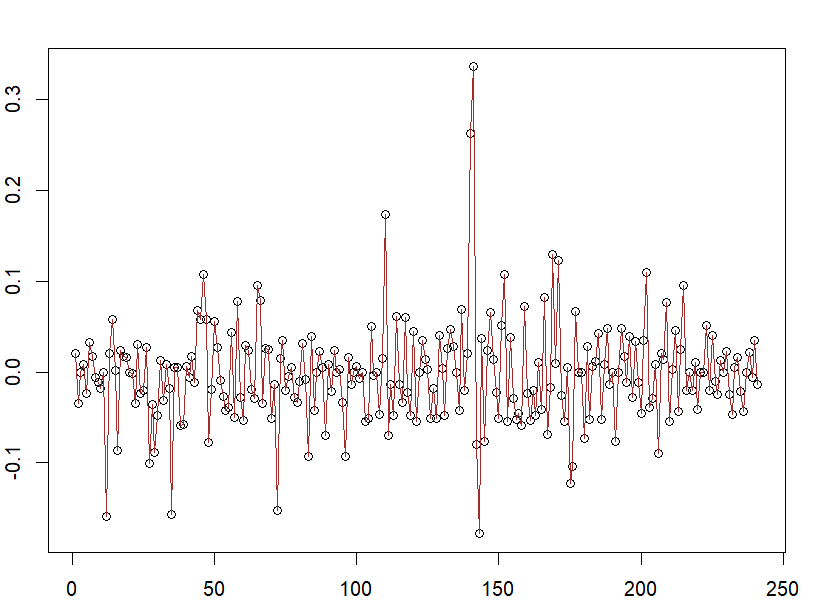
\includegraphics[width=10cm]{jjb_wykres_log.png}
        \label{fig:jjb_wykres_log}
	\caption{Wykres log-zwrotów spółki JJB}
\end{figure}

\begin{figure}[htb]
	\centering
	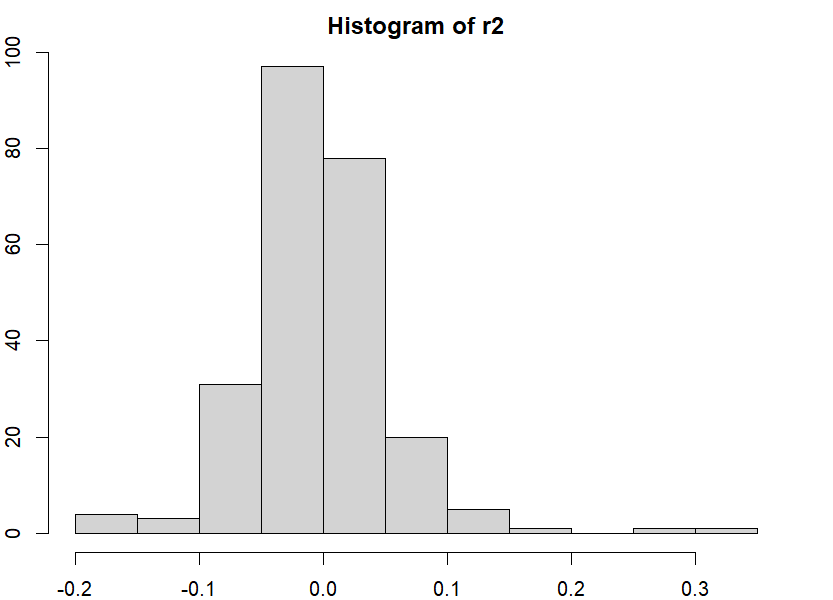
\includegraphics[width=10cm]{jjb_hist_log.png}
        \label{fig:jjb_hist_log}
	\caption{Wykres log-zwrotów spółki JJB}
\end{figure}

Został dopasowany do tych danych rozkład normalny $X \sim\ N(-0.0025,0.057 )$
\begin{figure}[htb]
	\centering
	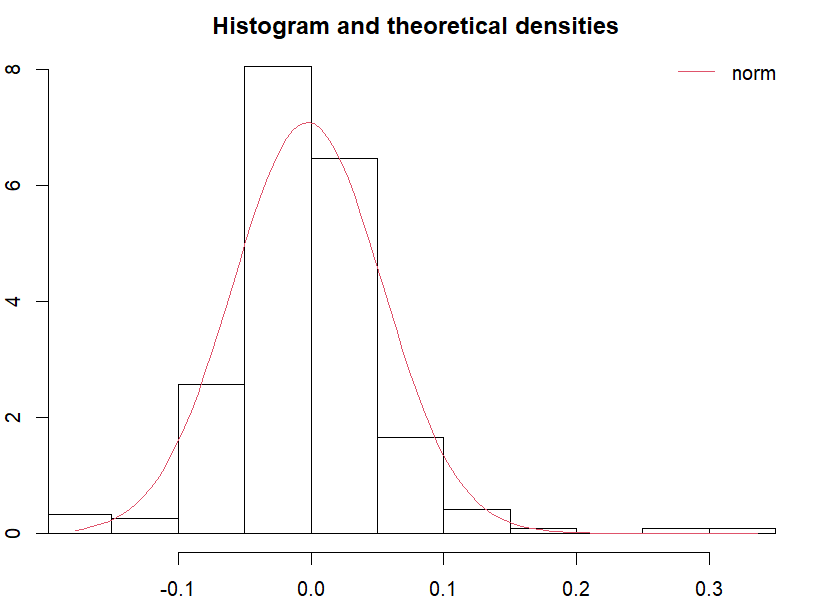
\includegraphics[width=10cm]{jjb_histwykres_log.png}
        \label{fig:jjb_histwykres_log}
	\caption{Wykres log-zwrotów wraz z dopasowanym rozkładem normalnym spółki JJB}
\end{figure}

Zrobiony wykres diagnostyczne cdf oraz qqplot, rysunki \ref{fig:jjb_qqplot_log}, \ref{fig:jjb_cdf_log.png}

\begin{figure}[htb]
	\centering
	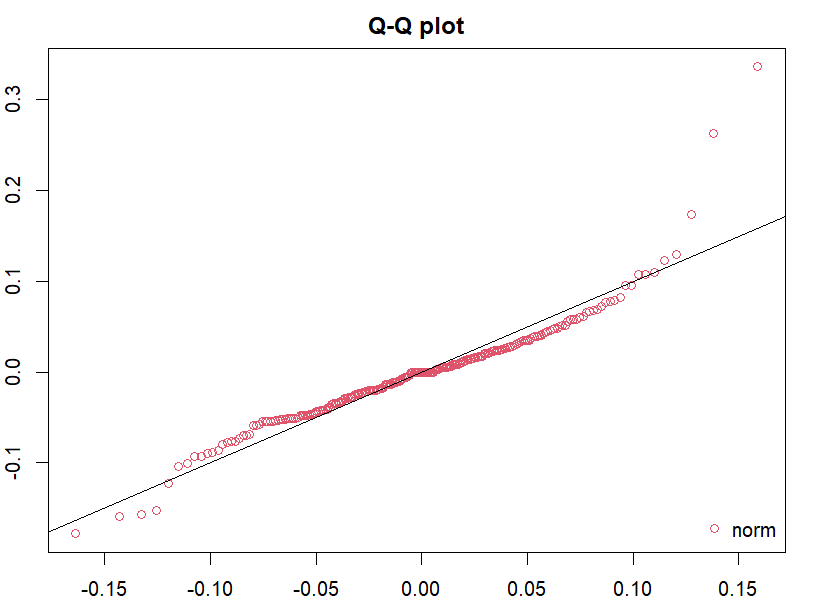
\includegraphics[width=10cm]{jjb_qqplot_log.png}
        \label{fig:jjb_qqplot_log}
	\caption{Wykres qqplot dla log-zwrotów spółki JJB}
\end{figure}

\begin{figure}[htb]
	\centering
	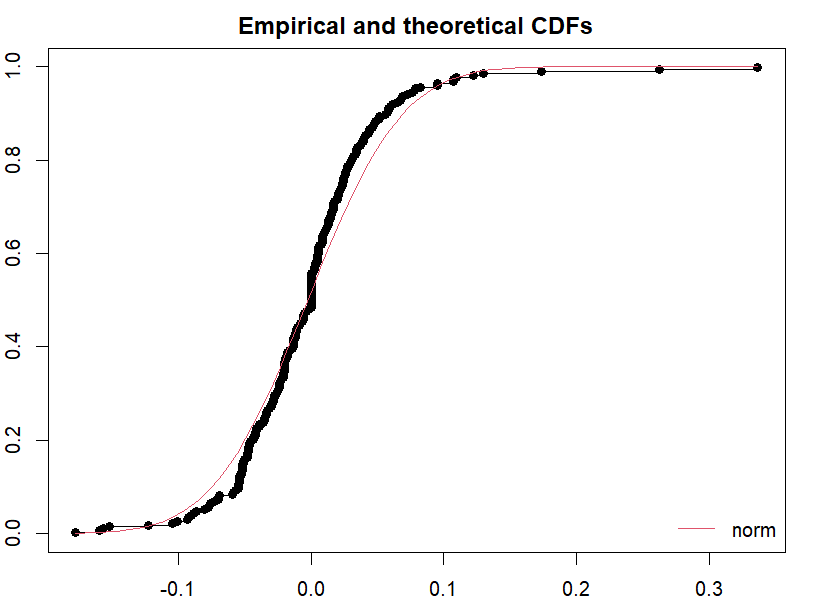
\includegraphics[width=10cm]{jjb_cdf_log.png}
        \label{fig:jjb_cdf_log.png}
	\caption{Wykres cdf dla log-zwrotów spółki JJB}
\end{figure}

Przeprowadzono również test równości metodą Monte-Carlo. Skorzystano ze statystyki Kolmogorova-Smirnova. Wynik p-value otrzymany w tym teście jest 0.5709, co oznacza przyjęcie hipotezy że rozklad log-zwrotów jest  $X \sim\  N(-0.0025,0.057 )$

\begin{figure}[htb]
	\centering
	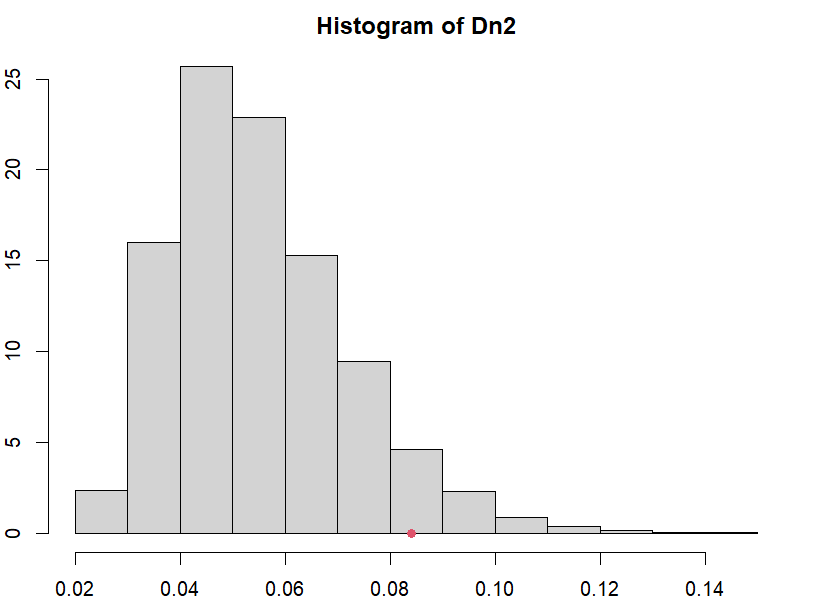
\includegraphics[width=10cm]{jjb_histMC.png}
        \label{fig:jjb_histMC}
	\caption{Histogram danych w teście }
\end{figure}



\subsection{Estymacja parametrów rozkładu dwuwymiarowego normalnego oraz analiza dobroci dopasowania}

Zrobiono wykres rozrzutu z histogramami brzegowymi, rysunek \ref{fig:wykres_rozrzutu}

\begin{figure}[htb]
	\centering
	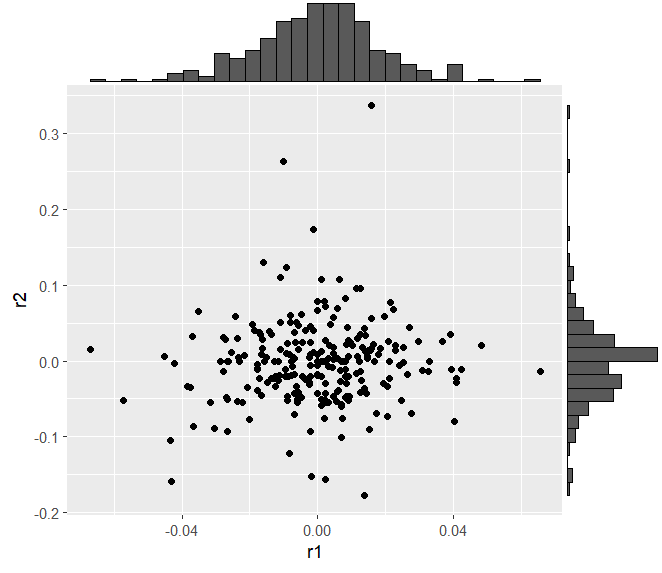
\includegraphics[width=10cm]{wykres_rozrzutu_histogram.png}
        \label{fig:wykres_rozrzutu}
	\caption{Wykres rozrzutu z histogramami brzegowymi}
\end{figure}

\subsubsection{Wykres rozrzutu z histogramami rozkładów brzegowych}
\subsubsection{Weltor średnich, kowariancji, macierz korelacji, współczynnik korelacji}
\subsubsection{Wzór gęstości rozkładu dwuwymiarowego normalnego}
\subsection{Analiza dopasowania rozkładu}
\subsubsection{Porównanie wykresów rozrzutu w oparciu o wygenerowaną próbę}
\subsubsection{Mahalanobis}
\end{document}